\section{Study 1: User Behavior on an Imaginary TypeBoard}

In this study, we collected data from participants' typing actions on a pressure-sensitive touchpad. The motivation was to investigate users' typing behavior on an imaginary touchscreen keyboard that prevents unintentional touch, based on which we could design the algorithm of unintentional touch prevention. Because (incorrect) feedback would affect users' behaviors, participants typed on a touchpad without any feedback in this study. Participants could not input words by typing. Instead, they imagined that the desired words are inputted. Besides, participants needed to adapt their behaviors according to the imagination that the keyboard can prevent unintentional touch.

\subsection{Participants}

We recruited 16 participants from the campus (aged from 19 to 26, M = 22.13, SD = 2.13, eight females). All the participants were right-handed and native Chinese speakers. They have used software keyboards on smartphones for not less than two years (M=7.50, SD = 2.25). Eight participants have ever used software keyboards on tablets.

\subsection{Design and Procedure}

Figure \ref{fig:study1_illu} illustrates the experimental setting. There was a Sensel Morph \cite{Website-Morph} pressure-sensitive touchpad on the desk. We placed a Windows Surface tablet computer on the touchpad, covering half of the touchpad. We drew a QWERTY layout on the touchpad using highlighter pens. The devices were a substitute for the pressure-sensitive touchscreen, which is not available in markets yet. Participants filled in a Microsoft Word document to complete the experimental tasks. They touched on the tablet to select table cell and typed on the touchpad to imagine inputting words. The system recorded every touch and the screencast during the experiment.

\begin{figure}[!tbh]
	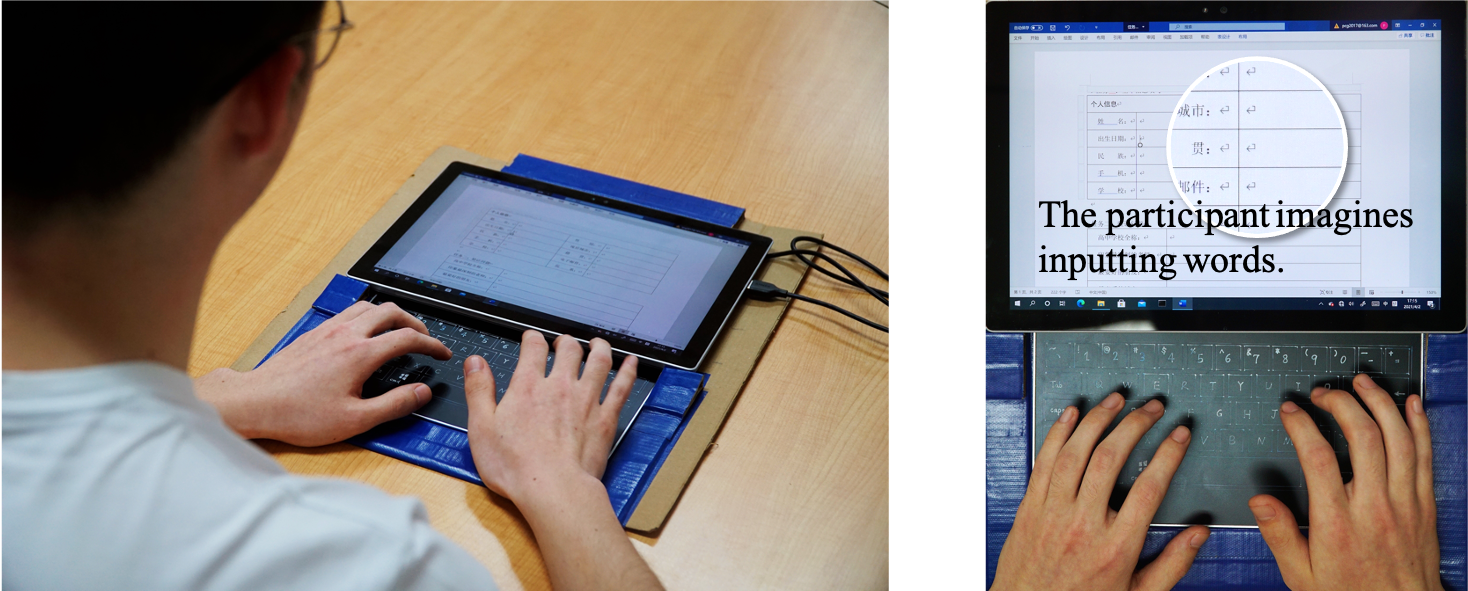
\includegraphics[width=0.9\linewidth]{figures/study1_illu.png}
	\centering
	\caption{The experimental setting of study one. We placed a tablet and a pressure-sensitive touchpad together as a substitute for the pressure-sensitive touchscreen. The keyboard had no feedback. The participant imagined inputting words.}
	\label{fig:study1_illu}
\end{figure}

The experiment included four text input tasks: (1) filling in personal information, (2) short questions, (3) open-book examination, and (4) picture writing. The tasks were in Chinese. We counterbalanced the order of tasks using a balanced latin square. We did not include transcription as a task as many other text entry studies do \cite{2003-Metrics, 2003-Phrase, 2017-Word}, because our pilot study showed that participants seldom rested their fingers on the touchpad in a transcription task, resulting in low efficiency of obtaining unintentional touches. The detail of tasks is as follows:

\begin{enumerate}
	\item{\textbf{Filling in personal information:} There was a table of ten blanks about personal information, such as name and gender. Figure \ref{fig:study1_task}(a) shows the examples in Chinese and the corresponding translation. This assignment represented those tasks that require frequent switching between text input and cursor control. To protect privacy, participants felt free to fill in fake information. However, participants should remember what they intended to input, which is crucial for the subsequent process of labeling data.}
	\item{\textbf{Short questions:} There was a table of ten short questions, such as "the favorite color" and "the best friend". Participants were allowed to fill in a fake answer.}
	\item{\textbf{Open-book examination:} The exam consisted of five hard questions, such as "what is the 50th element on the periodic table?". Participants could hardly know the answers, so they needed to search the Internet. This assignment represented the common task of browsing websites. Because the participants could not input words in the search engine, they said as they wrote, so the experimenter could replace them to input the words.}
	\item{\textbf{Picture writing:} As figure \ref{fig:study1_task}(b) shows, participants described the picture in five sentences. This assignment represented the tasks of writing articles. Participants said as they wrote, so the experimenter could replace them to input the words.}
\end{enumerate}

\begin{figure}[!tbh]
	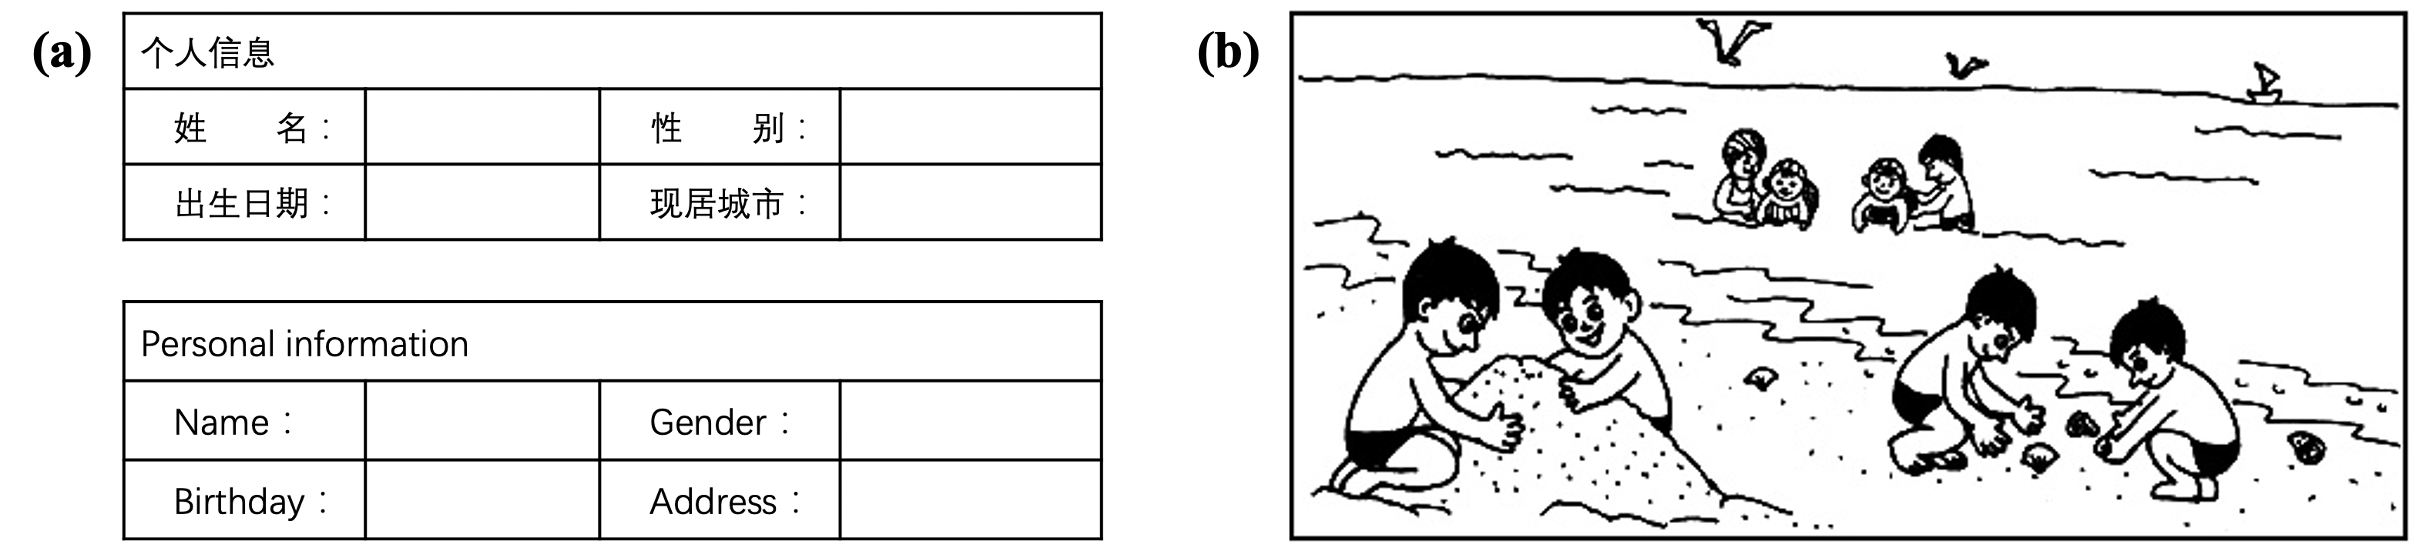
\includegraphics[width=0.9\linewidth]{figures/study1_task.png}
	\centering
	\caption{The illustration of experimental tasks. The left side shows the examples of task one (filling in personal information) in both Chinese and translation. The right side is the figure we used in task four (picture writing).}
	\label{fig:study1_task}
\end{figure}

Before the experiment, the participant had five minutes to get familiar with the experimental requirement. In the warm-up phase, participants typed on the touchpad freely. We reminded the participants of two points. First, the keyboard did not provide any feedback. Participants could not input words but imagined inputting words. As the Chinese text entry method involved word selection, participants assumed that the desired word is always the first in the candidate list. Second, users needed to imagine that the keyboard prevents unintentional touches and adjust their behavior according to this assumption. For example, they could rest their fingers on the keyboard while thinking.
%This is not mandatory. Participants could make choices as they wished.

%在实验开始前,用户有5分钟的时间自由地在本系统中熟悉实验的任务和要求,在热身的过程中,实验者让用户注意两点:第一,本实验的键盘不会提供任何反馈,用户不能键入字母,而是想象自己键入了字母。由于用户的母语是中文,在输入的过程中会涉及到选词,用户只需想象想要的单词总是在输入法候选词的第一位。第二,用户需要想象该键盘可以完美地防误触,并根据这一条件调整自己的输入行为,比如,在思考问题的时候可以将手指休息在键盘上。这种行为调整不是强制性的,用户可以根据自己的实际情况作出选择。

\begin{figure}[!tbh]
	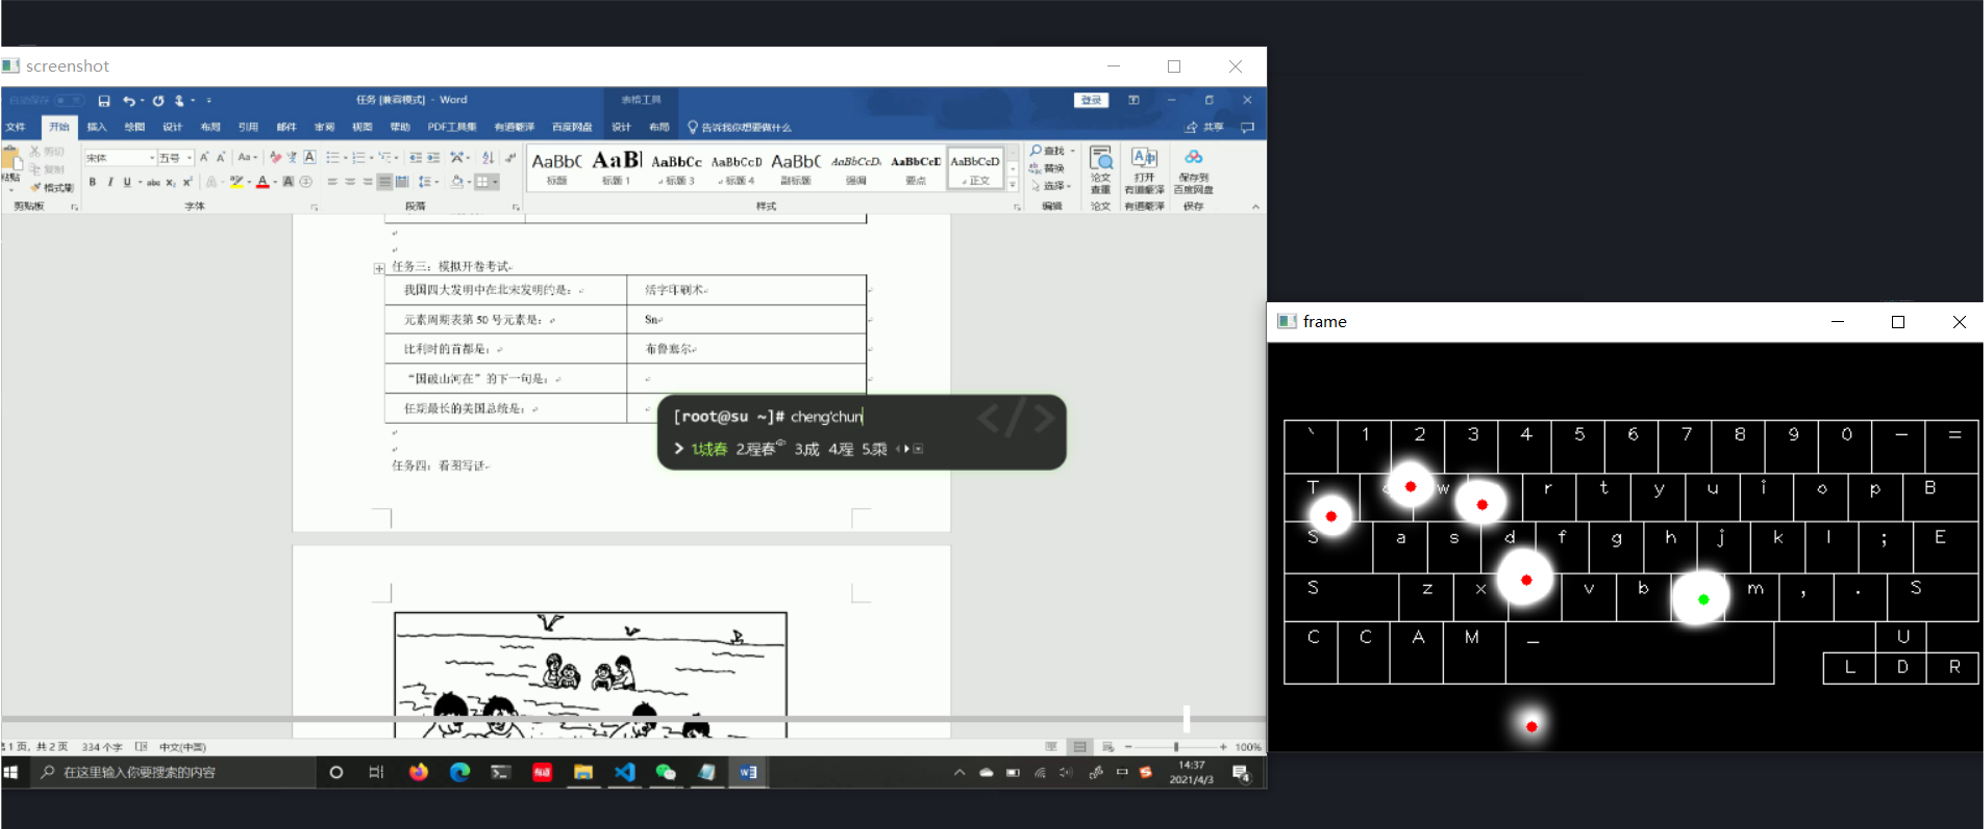
\includegraphics[width=1.0\linewidth]{figures/label_process.png}
	\centering
	\caption{The illustration of the label program.}
	\label{fig:label_process}
\end{figure}


After each task, the participant labeled the data through an interactive program as figure \ref{fig:label_process} shows. The program showed the touchpad capacitive images and the tablet screencast at the same time. There were red points on capacitive images that showed the touchpoints. Participants labeled the intended touches as green points. Participants were able to judge most touches because they could get context from the screencast. If participants were not sure, they labeled the touchpoints as blue points to remove the data. On average, participants spent five minutes finishing the text input tasks and spent 45 minutes labeling the data. Participants rested for five minutes between two tasks to avoid fatigue. The study lasted for 70 minutes.

\subsection{Apparatus}

As figure \ref{fig:study1_illu}(right) shows, we placed a Windows Surface tablet computer and a Sensel Morph pressure-sensitive touchpad \cite{Website-Morph} together as a substitute for the pressure-sensitive touchscreen. The Sensel Morph senses the position and the pressure level of touches. The Sensel Morph contains 185 x 105 sensor elements ("sensels") at a 1.25mm pitch. Each contact can sense approximately 30000 levels, ranging from 5g to 5kg. The maximal frequency of the Sensel Morph was 125Hz (8ms latency). We slowed the frequency down to 50Hz to fetch stable data. The Sensel Morph provides capacitive images and touchpoint information, including position, timestamp, touch area, pressure level, and shape. The device is so sensitive that almost every touch is recognized. Thus, in this paper, we identified unintentional touches among reported touchpoints while ignoring the Sensel Morph's missing touches.

The size of the sensing area on the Sensel Morph was 240 mm x 138 mm. We used highlighter pens to draw a Qwerty layout on the touchpad. The Sensel Morph width (240mm) was shorter than the keyboard on a 15 inches MacBook (270mm). We removed some keys that are less frequently used, such as square brackets and the semicolon, so that the Qwerty layout could be placed in the Sensel Morph, while each key's size remained the same as Macbook. Because the Qwerty layout is changeable in the software keyboard, we did not leverage the layout as prior knowledge to recognize unintentional touch. The tablet computer was Windows Surface Pro6, with i7 Intel Core Processor. The program ran on the tablet at 50 FPS.

\subsection{Result}

The dataset contains 12659 touches, excluding the ambiguous touches (0.18\%) in the labeling process. 67.5\% of the data were positive samples (intentional touches), while 32.5\% were negative samples (unintentional touches). Based on the data, we developed the TypeBoard in three steps, each contributing to solving one of the critical problems as follows:

\begin{enumerate}
	\item{\textbf{Model V1):} \emph{data processing.} There were some mislabeled data points because some participants misunderstood the concept of unintentional touches. We developed a naive Support Vector Machine (SVM) model to identify unintentional touch. If there was a vast difference between the predicting results and the labels, we asked the participants to relabel the suspicious data points through e-mails.}
	\item{\textbf{Model V2):} \emph{filtering multiple fingers resting.} Observation suggested that multiple fingers resting was the most frequent unintentional touch, where users rested more than two fingers on the screen. We added targeted criteria into the SVM model to filter out multiple fingers resting.}
	\item{\textbf{Model V3):} \emph{understanding the user behavior.} We analyzed the fail cases of Model \textbf{V2} to understand those user behaviors that challenged the algorithm, based on which we further improved the SVM model.}
\end{enumerate}

\begin{table}[!tbh]
	\caption{The features we fed into the SVM model and the accuracy among model versions. For the features except "the relationship to recent/nearby touches", we extracted the temporal features over frames, including maximum, minimum, mean, skewness, and kurtosis.}
	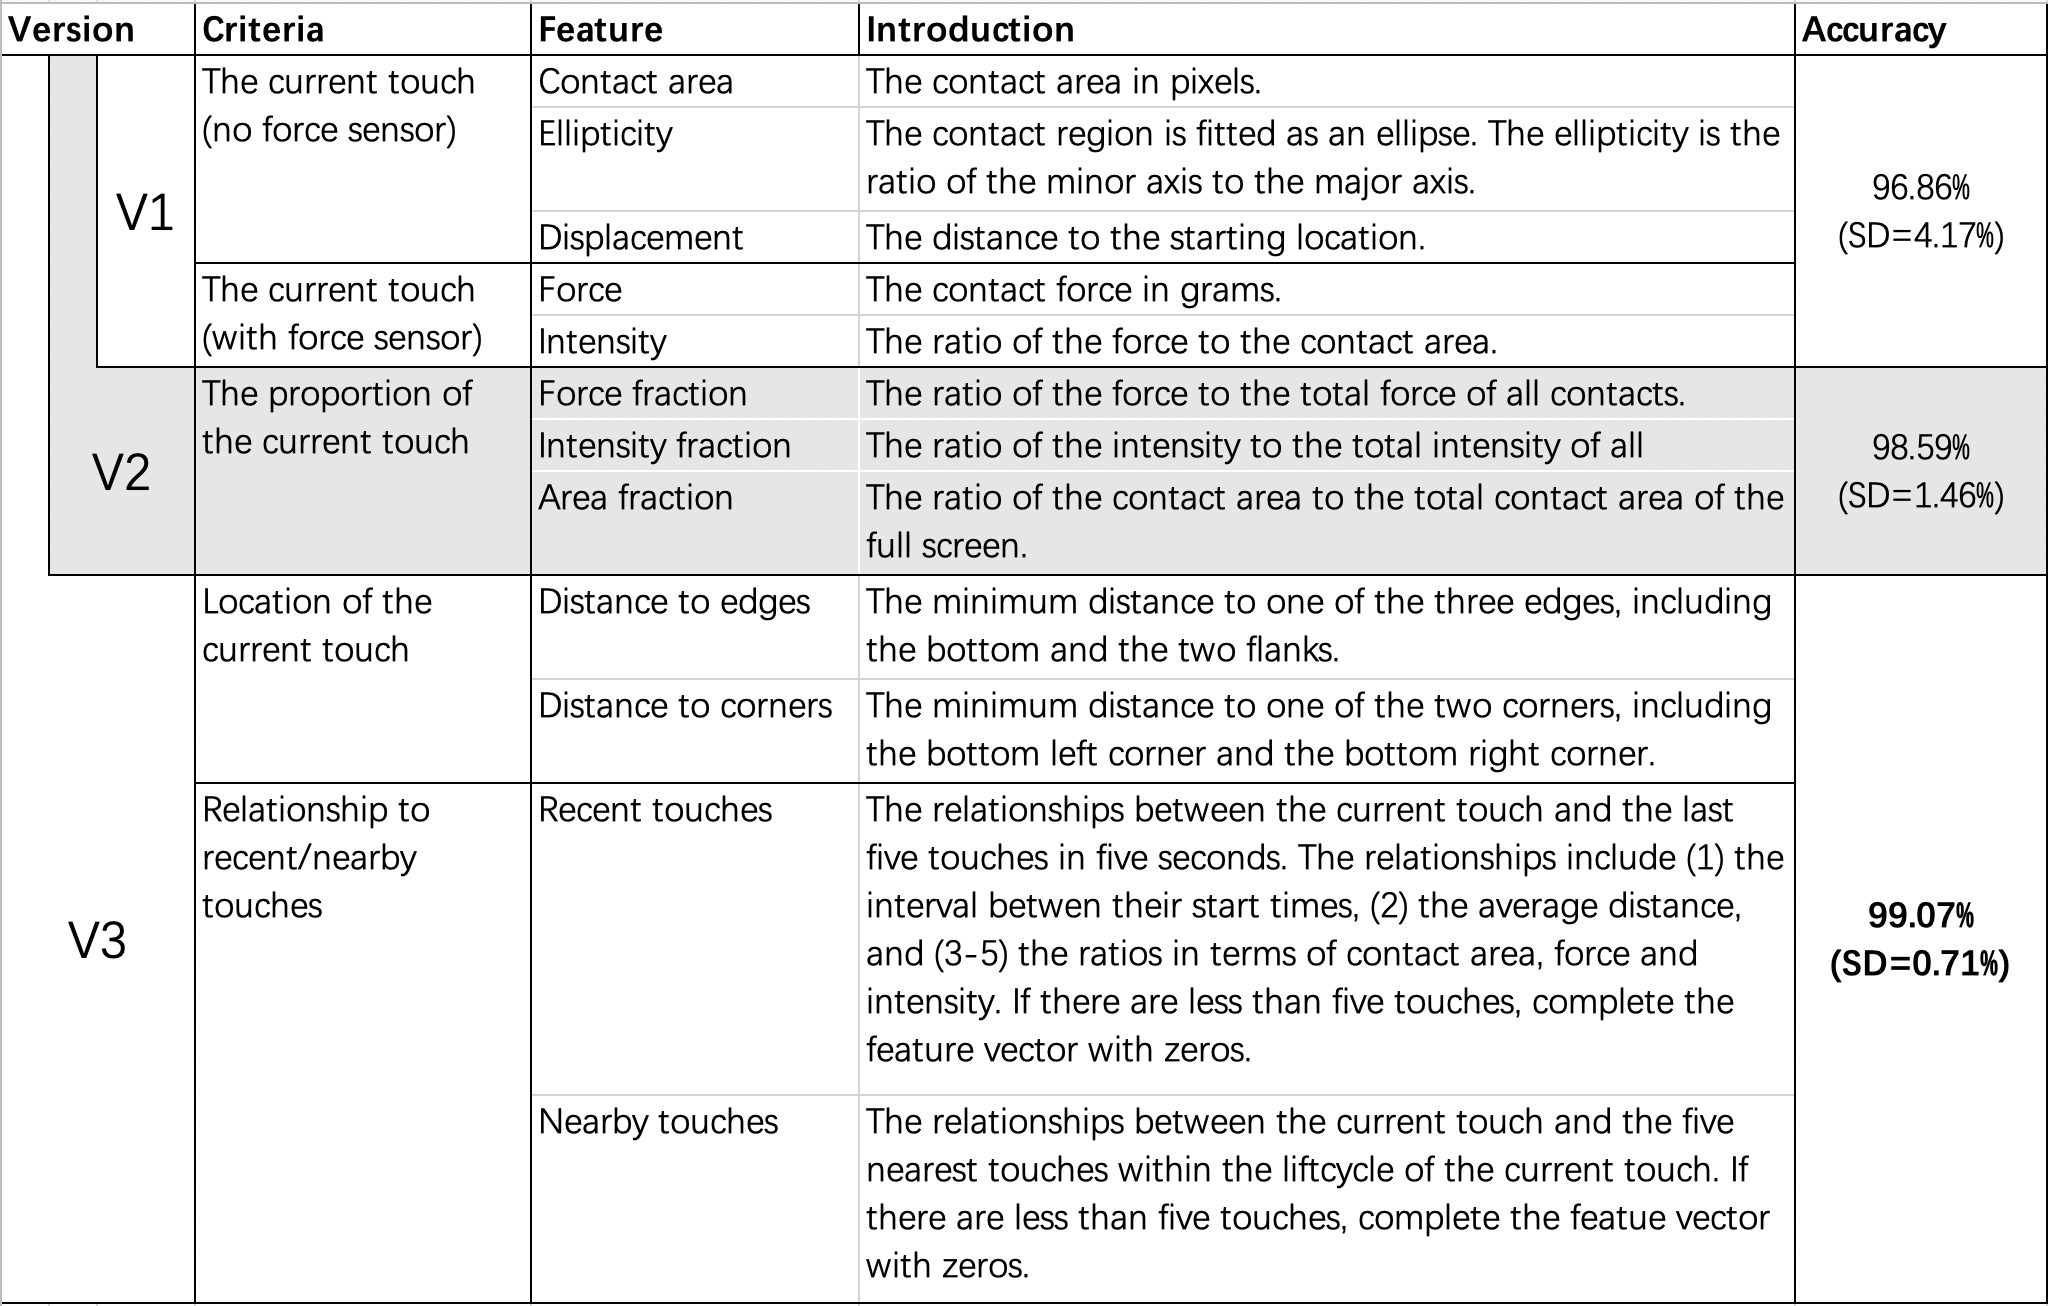
\includegraphics[width=1.0\linewidth]{figures/features.png}
	\centering
	\label{tab:study_features}
\end{table}

Table \ref{tab:study_features} shows the feature vector we used to train the SVM model in each step and the recognition results. In the remainder of this subsection, we introduced the unintentional touch identification model in detail.

%Because some participants misunderstood the concept of unintentional touches when labeling, there were some mislabeled data points. We trained a simple machine learning model (version 1) to process the data. If there were too many differences between the labels and the predicting results, we asked the participants to relabel the suspicious data points.

\subsubsection{Model  V1: naive model for data processing}

In the first step, we trained a naive SVM model to identify unintentional touch using straightforward features. We sampled the first five frames (100 ms) of each touch. If the touch duration is shorter than five frames, we sampled the whole touch. As table  \ref{tab:study_features} (\textbf{V1}) shows, we extracted features from the samples as follows: for the contact area, ellipticity, displacement, force, and intensity over frames, we calculated the temporal features, including maximum, minimum, mean, skewness, and kurtosis. Then, we concatenated these values to obtain a feature of 25 dimensions and trained an SVM binary classifier, namely Model \textbf{V1}. We balanced positive and negative samples in weight.

We used the model to simulate the dataset. We found that some participants misunderstood the concept of unintentional touches, for example, regarding incorrect character inputs as unintentional touches. We asked the participants to relabel the suspicious data points through e-mail. After the label correction, we had 12624 data points, including 68.38\% positive samples and 31.62\% negative samples. Leave one out cross-validation shows that the accuracy of Model \textbf{V1} was 96.86\% (SD=4.17\%). 

%For comparison, if we did not have the force signal (i.e., the regular touchscreen devices), the accuracy would reduce to 92.30\% (SD=4.88\%). The result shows that the force signal is important for unintentional touch rejection (F,p).

\subsubsection{Model V2: filtering multiple fingers resting}

Observation showed that most unintentional touches (72.66\%) were caused by multiple fingers resting, where users rested no less than three fingers on the screen simultaneously. The resting fingers contact the screen one after another. After the first touch, the following touches come within 100 ms in most instances. In 86.05\% cases, the second finger touches within 100 ms, while in 76.30\% cases, the third finger also touches within 100 ms. Because our model has a latency of 100 ms, the model has a big chance to realize that multiple fingers are resting. Thus, we could design targeted features to filter out the unintentional touches caused by multiple fingers resting.
We added a series of features in Model \textbf{V2} to deal with this problem. The criterion was the proportion of the touch's pressure, intensity, and contact area among all touches. Table \ref{tab:study_features} (\textbf{V2}) shows the details. Leave one out cross-validation shows that Model \textbf{V2} increased the recognition accuracy to 98.59\%.

\subsubsection{Model V3: understanding the user behavior to  improve the model}

We analyzed the fail cases of Model \textbf{V2} to understand those user behaviors that challenged the model. The error rate of Model \textbf{V2} was 1.41\%, including 1.00\% false positives and 0.41\% false negatives. The false positives referred to the misrecognized unintentional touches, while the false negatives were the missing intentional touches. As table \ref{tab:fail_cases} shows, we classified the fail cases into 16 categories. We counted each kind of fail case, discussed the reasons, and gave possible solutions. For the fail cases with a white background in the table, humans (the researchers) could judge their intentions without extracting contextual information from the experiment screencast. That is, the machine should have correctly predicted if it is as smart as a human. For these cases, we proposed features to improve the model. Here are some examples.

\begin{enumerate}
	\item{\textbf{EG1):} \emph{Hypothenar eminence.} As figure \ref{fig:fail_case_examples}(a) shows, the hypothenar eminence refers to a group of muscles of the palm that control the motion of the little finger, while the thenar eminence is the group of muscles on the palm at the base of the thumb. Both the two eminences may contact the touchscreen when a user is typing. In particular, the touches caused by the hypothenar eminence are usually heavy and intensive, which is easy to confuse with intentional touches. Fortunately, these touches are in the bottom left and the bottom right corners. Thus, the distance to the closest corner could be a powerful feature to reject these unintentional touches.}
	\item{\textbf{EG2):} \emph{Continuous touches.} When a user continuously typed on the same key (e.g., the backspace), the following touches were lighter than the first touch (p < 0.005). Among the continuous touches, the average pressure of the first touch was 167.01 g (SD = 106.76), while the average pressure of the following touches was 150.42 g (SD = 112.70). Because the following touches are light, they are likely to be recognized as unintentional touches. Information of recent touches help to correct this fail case.}
	\item{\textbf{EG3):} \emph{One-hand typing.} As figure \ref{fig:fail_case_examples}(b) shows, sometimes the participant typed with one hand while resting the other hand on the touchscreen. In this situation, the Model \textbf{V2} mistakenly believed that all the touches were unintentional touches caused by the multiple fingers resting behavior. We added information of nearby touches to correct this fail case because the typing finger is usually far away from the resting fingers.}
\end{enumerate}

\begin{figure}[!tbh]
	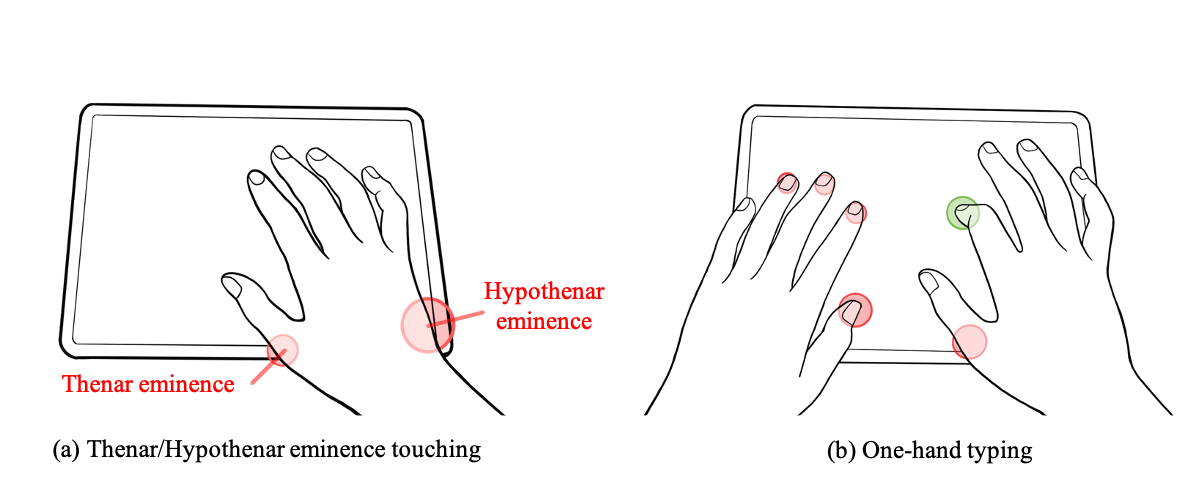
\includegraphics[width=1.0\linewidth]{figures/fail_case_examples.png}
	\centering
	\caption{The examples of fail cases. The fail cases reveal those user behaviors that challenged the algorithm.}
	\label{fig:fail_case_examples}
\end{figure}

% Table generated by Excel2LaTeX from sheet '写在论文中的中等粒度分类'
\begin{table}[htbp]
  \centering
  \caption{The fail cases of Model \textbf{V2}. The "N" column refers to the counting of each case.}
    \begin{tabular}{|p{8.5em}|p{21em}|r|p{10.5em}|}
    \toprule
    \textbf{Cases} & \textbf{Introduction} & {\textbf{N}} & \textbf{Helpful features?} \\
    \midrule
    \rowcolor[rgb]{ 1,  .902,  .6} \multicolumn{4}{|l|}{\textbf{False Positives}} \\
    \midrule
    Hypothenar eminence (figure \ref{fig:fail_case_examples}a) & The hypothenar eminence usually contacts the screen while typing. & 23    & Touchpoint location, e.g., nearing the corners? \\
    \midrule
    Thenar eminence (figure \ref{fig:fail_case_examples}a) & The thenar eminence usually contacts the screen while typing. & 2     & Touchpoint location, e.g., nearing the bottom edge? \\
    \midrule
    Repeated reporting (spatial) & A touch is misrecognized as two touches when the contact area is large. & 12    & Info. of nearby touchpoints. \\
    \midrule
    Repeated reporing (temporal) & A touch is misrecognized as two touches if the touch is nearly released midway. & 3     & Info. of recent touchpoints. \\
    \midrule
    Edge touch & Users trigger unintentional edge touch when adjusting the placement of devices. & 7     & Touchpoint location, e.g., nearing the flanks? \\
    \midrule
    Two fingers resting & The user rests two fingers on the screen. & 3     & Info. of nearby touchpoints. \\
    \midrule
    Extra touchpoint (light) & When inputting, users trigger extra touchpoints, which are lighter than the recent intentional touches. & 9     & Is this touch lighter than the recent touches? \\
    \midrule
    Slide & A slide is less likely to be an intentional keystroke. & 7     & Touchpoint displacement. \\
    \midrule
    \rowcolor[rgb]{ .949,  .949,  .949} One finger resting & Users rest one finger on the touchsreen, which is indistinguishable from an intentional touch. & 9     & No solution. \\
    \midrule
    \rowcolor[rgb]{ .949,  .949,  .949} Extra touchpoint (heavy) & When inputting, users trigger extra touches heavily, which seems like an intentional touch. & 15    & No solution. \\
    \midrule
    \rowcolor[rgb]{ 1,  .902,  .6} \multicolumn{4}{|l|}{\textbf{False Negatives}} \\
    \midrule
    Continuous touches & When a user continuously type on the same key (e.g., the delete key), the following touches will be lighter. & 13    & Info. of recent touchpoints. \\
    \midrule
    Rollover-typing & The next key is pressed before the previous is released \cite{2018-Observations}. & 12    & info. of recent touchpoints. \\
    \midrule
    One-hand typing & The user types with one hand, while the other hand is resting on the screen. This case is similar to multiple fingers resting. & 6     & info. of nearby touchpoints. \\
    \midrule
    Palm touch & The use types a key when the palm is resting on the screen. If the palm touch is detected as multiple fingers, this case is similar to multiple fingers resting. & 5     & info. of nearby touchpoins, e.g., is this touch near other touches? \\
    \midrule
    \rowcolor[rgb]{ .949,  .949,  .949} Light touch & The very light but intended touch, which is indistinguishable from an unintentional touch. & 46    & No solution. \\
    \midrule
    \rowcolor[rgb]{ .949,  .949,  .949} Small contact area & The intended touch with a very small contact area. This seems like an unintentional touch. & 6     & No solution. \\
    \bottomrule
    \end{tabular}%
  \label{tab:fail_cases}%
\end{table}%

However, for the fail cases with gray background in table \ref{tab:fail_cases}, humans (the researchers) could judge their intentions without watching the experiment screencast. We deemed that these fail cases are inevitable because the machine can not know what the user will input in advance. Here are some examples. First, sometimes the participant rested one finger on the touchscreen heavily, indistinguishable from an intentional touch. Second, the participant performed a very light touch during inputting a word, which is indistinguishable from an unintentional touch. Thus, the model's accuracy has a certain upper limit (roughly 99.40\% in this dataset), while our goal is to approach it.

According to the user behaviors summarized in table \ref{tab:fail_cases}, we added two criteria in the model training. The first one is the location of the touch, including the minimum distances to the edges and the corners. We did not leverage the prior knowledge of the keyboard layout because the software keyboard layout is changeable, while we wanted a universal model. The second criterion is the relationships between the current touch and the recent/nearby touches. The features in detail are in table \ref{tab:study_features} (\textbf{V3}). The Model \textbf{V3} used all the features in the table. We concentrated these features to form a vector of 100 dimensions and trained an SVM binary classifier. Leave one out cross-validation showed that the accuracy was 99.07\%. The error rate was 0.93\%, including 0.56\% false positives and 0.37\% false negatives. So far, we have obtained a model with high recognition accuracy. However, as we said in the introduction, the data collected in study one did not represent the user behavior on the software keyboard with unintentional touch prevention, so we named Model \textbf{V3} as semi-finished TypeBoard. In study two, we collected the user behavior on the semi-finished TypeBoard and then used the new data to improve the model.

% We used previous work as baseline \cite{2013-TapBoard}, where every touches that last for more than 450 ms or move father than 15 mm are identified as unintentional touches. We adjusted the thresholds to yy ms and yy mm so that the baseline performed the best on our dataset. Our result (99.07\%) surpassed the baseline (yy\%). In real use, our system calls the classifier once a touch has lasted for five frames or is released in advanced. The system reports the touchpoint if the prediction result is positive. The delay of our method is 100 ms. For comparison, the baseline can only judge a touch when it is released.

%We have three conclusions in this experiments. First, participants were willing to rest their fingers on the touchscreen that can reject unintentional touches in imaginary. Hereby, we proposed a hypothesis to be verified, where users are willing to rest their fingers on a real TypeBoard. Second, the force signal is important for rejecting unintentional touches in the text entry task. Third, most unintentional touches (>99\%) can be identified by spatial-temporal features of the signals on a force-sensitive touchsreen keyboard.

